% Provenance (never printed): see sources/outline_sources.md (Year 3:
% geomorphology, hillslope processes, river incision, landscape evolution).
% Brief: sources/book5/BRIEFS.md, ch. 18. Curves from
% figdata/bachelor-3/hillslope.py, stream_profile.py and varden_river.py.
% Exercise and problem values in the Book 5 scratch calculator calc/ch18.py.
% The upland west of the Varden Hills, its river, its tributaries, its
% uplift rate and its base-level fall are invented; the outlet elevation is
% the region model's river at the west edge of the map.
\chapter{परिमाणात्मक भूआकृति विज्ञान}\label{ch:b3:quantitative-geomorphology}

उभरती परास को पार करती एक नदी की अनुदैर्ध्य परिच्छेदिका में एक सोपान होता है: एक जलप्रपात,
जिसके नीचे एक गॉर्ज और ऊपर एक अपेक्षाकृत मंद घाटी होती है। सोपान अपने बनने के स्थान पर
नहीं टिकता। वह ऊपरी धारा की ओर चढ़ता है, कुछ मिलीमीटर या कुछ मीटर प्रति
वर्ष, और उसकी स्थिति एक ऐसी घड़ी है जो तब चली जब नदी का \omterm{def:b3:quantitative-geomorphology:knickpoint}{आधार-तल}
नीचे गिराया गया। उस घड़ी को पढ़ना, और ढालों तथा नदियों के आकारों में लिखी
दरों को पढ़ना दो संरक्षण नियम और दो परिवहन नियमों की माँग करता है: एक उस मिट्टी के लिए
जो ढलान पर नीचे सरकती है, और एक उस आधार-शैल के लिए जिसे नदी काटती है।

\begin{recall}
अपक्षय, अपरदन, निक्षेपण, भूरूप, और उत्थान तथा अपरदन के बीच का संतुलन
विद्यालय स्तर की पुस्तकों में हैं, जैसे समस्थितिक प्रतिक्षेप और U-आकार की
हिमनदीय घाटियाँ। अनाच्छादन दर, तल कर्तन-प्रतिबल और शील्ड्स
प्राचल पुस्तक 3 (स्नातक वर्ष 1) में हैं, उसके अपरदन और परिवहन वाले अध्याय में;
अंकीय उन्नयन मॉडल उसके भूवैज्ञानिक मानचित्र वाले अध्याय में, और एयरी
समस्थिति उसके समस्थिति और गुरुत्व विसंगति वाले अध्याय में। \omterm{def:b3:advanced-geochronology:cosmogenic}{ब्रह्मांडजनित
नाभिक} और उनसे प्राप्त अपरदन दरें
अध्याय~\ref{ch:b3:advanced-geochronology} में हैं, और \omterm{def:b3:orogenic-wedges:thermochronology}{ऊष्मकालमिति} तथा \omterm{def:b3:orogenic-wedges:age-elevation}{आयु--ऊँचाई संबंध}
अध्याय~\ref{ch:b3:orogenic-wedges} में।
यह विसरण समीकरण भौतिकी की पुस्तकों में है।
\end{recall}

\section{ढाल}\label{sec:b3:quantitative-geomorphology:hillslopes}

मिट्टी से ढकी एक पहाड़ी पर मिट्टी कण-दर-कण ढलान की ओर खिसकती है: बिल खोदने वाले
जीव उसे उछालते हैं, जड़ें उसे उभारती हैं, जमना और भीगना उसे फुलाते हैं, और हर
विक्षोभ गुरुत्व को उसे थोड़ा खिसकाने देता है। सदियों पर औसत करें तो मिट्टी का
फ़्लक्स ढलान के समानुपाती होता है।

\begin{definition}[ढाल विसरण]\label{def:b3:quantitative-geomorphology:diffusion}
\emph{ढाल विसरण}\index{ढाल विसरण} मिट्टी का धीमा, ढलान की ओर होने वाला परिवहन है
जिसका ढाल की प्रति इकाई चौड़ाई पर आयतन फ़्लक्स,
$\vec q$, सतह की ऊँचाई $z$ की प्रवणता के समानुपाती है:
$\vec q = -\kappa\,\nabla z$। गुणांक $\kappa$, जो
\unit{m^2/yr} में मापा जाने वाला यह गुणांक ढाल विसरणशीलता है।
\end{definition}

\begin{theorem}[ढालों का विसरण]\label{thm:b3:quantitative-geomorphology:diffusion}
मान लीजिए कि चट्टान उस ढाल को सीमित करने वाली वाहिकाओं के सापेक्ष दर $U$ से
उठ रही है, मिट्टी और चट्टान का घनत्व समान है, और मिट्टी \omterm{def:b3:quantitative-geomorphology:diffusion}{ढाल विसरण} से
एकसमान $\kappa$ के साथ खिसकती है। तब सतह की ऊँचाई निम्न समीकरण का पालन करती है:
\[
\frac{\partial z}{\partial t} = U + \kappa\,\nabla^2 z ,
\]
यह स्रोत पद वाला विसरण समीकरण है।
\end{theorem}

\begin{proof}
ढाल का एक छोटा क्षेत्र $\delta S$ लीजिए। उसका आयतन उत्थान के कारण
प्रति इकाई समय $U\,\delta S$, और उसकी किनारों से बाहर बहने वाली मिट्टी से
बदलता है: $\oint \vec q\cdot\vec n\,\mathrm{d}\ell = (\nabla\cdot\vec q)\,\delta S$।
अतः $\partial z/\partial t = U - \nabla\cdot\vec q$ प्राप्त होता है; जहाँ $\vec q = -\kappa
\nabla z$ और $\kappa$ एकसमान है, $\nabla\cdot\vec q = -\kappa\nabla^2 z$।
\end{proof}

कोई भ्रंश या तटरेखा एक ही क्षण में कगार काटती है; उसके बाद कगार केवल
विसरित होता है। अर्ध-ऊँचाई $a$ के एक ऊर्ध्वाधर सोपान से, जो
दूर-क्षेत्र की ढाल $b$ पर है, एक-विमीय हल यह है
\[
z(x,t) = a\,\operatorname{erf}\!\left(\frac{x}{2\sqrt{\kappa t}}\right) + b\,x ,
\qquad
\left.\frac{\partial z}{\partial x}\right|_{x=0} = \frac{a}{\sqrt{\pi\kappa t}} + b .
\]
आकार केवल गुणनफल $\kappa t$ पर निर्भर करता है: एक मापी गई परिच्छेदिका से
$\kappa t$ प्राप्त होता है; या तो एक स्वतंत्र आयु से $\kappa$ मिलता है, या ज्ञात
$\kappa$ से आयु मिलती है, जिसे \emph{आकारिकीय आयु} कहते हैं। अर्ध-शुष्क
क्षेत्रों में, जहाँ कणिकामय मिट्टी और विरल वनस्पति है, कगार $\kappa$ का मान
$10^{-3}$ और \qty{e-2}{m^2/yr} के बीच; आर्द्र, घनी वनस्पति वाले तटीय पर्वतों में
लगभग \qty{5e-3}{m^2/yr} है।
% ledger: whipple04:scarp-erf, whipple04:scarp-kappa

\begin{omfigure}
\begin{tikzpicture}
\begin{groupplot}[group style={group size=2 by 1, horizontal sep=1.6cm},
  width=0.48\linewidth, height=0.36\linewidth, tick label style={font=\scriptsize},
  label style={font=\small}, legend style={font=\scriptsize, draw=none, fill=none}]
\nextgroupplot[xlabel={दूरी $x$ (m)}, ylabel={$z$ (m)}, xmin=-40, xmax=40,
  ymin=-5, ymax=5, legend pos=north west]
% computed in figdata/bachelor-3/hillslope.py
\addplot[black!50, densely dashed] table[x=x, y=z0] {figdata/out/bachelor-3-hillslope-scarp.dat};
\addplot[omDef, thick] table[x=x, y=z1] {figdata/out/bachelor-3-hillslope-scarp.dat};
\addplot[omProp, thick] table[x=x, y=z2] {figdata/out/bachelor-3-hillslope-scarp.dat};
\addplot[omThm, thick] table[x=x, y=z3] {figdata/out/bachelor-3-hillslope-scarp.dat};
\legend{आरंभिक, \qty{2}{kyr}, \qty{10}{kyr}, \qty{40}{kyr}}
\nextgroupplot[xlabel={विभाजक से दूरी (m)}, ylabel={ऊँचाई (m)},
  xmin=-150, xmax=150, ymin=0, ymax=200, xtick={-150,-75,0,75,150}]
\addplot[omMeth, thick] table[x=x, y=z1] {figdata/out/bachelor-3-hillslope-hill.dat};
\addplot[omDef, thick] table[x=x, y=z2] {figdata/out/bachelor-3-hillslope-hill.dat};
\addplot[omThm, thick] table[x=x, y=z3] {figdata/out/bachelor-3-hillslope-hill.dat};
\node[font=\scriptsize, anchor=north] at (axis cs:0,45) {0.0215};
\node[font=\scriptsize, anchor=north] at (axis cs:0,94) {0.043};
\node[font=\scriptsize, anchor=north] at (axis cs:0,184) {\qty{0.086}{mm/yr}};
\end{groupplot}
\end{tikzpicture}

\par\smallskip{\small बाईं ओर, \qty{5}{m} विस्थापन वाला एक कगार, जो
0.05 की ढाल पर है, $\kappa = \qty{5e-3}{m^2/yr}$ के साथ विसरित हो रहा है: आरंभिक सोपान
(बिंदीदार) और 2, 10 तथा \qty{40}{kyr} के बाद की परिच्छेदिकाएँ। दाईं ओर, स्थायी
पहाड़ियाँ, अर्ध-चौड़ाई \qty{150}{m} की, उसी $\kappa$ के साथ (वाहिकाओं से ऊपर
की ऊँचाई), जो घट रही हैं
0.0215, 0.043 और \qty{0.086}{mm/yr} की दरों से: परवलय, जिनका उच्चावच और शिखर पर वक्रता
अपरदन दर के समानुपाती हैं।}\label{fig:b3:quantitative-geomorphology:hillslope}
\end{omfigure}
% ledger: whipple04:scarp-kappa

जब कोई पहाड़ी लंबे समय तक उत्थान और अपरदन से गुज़रती है, तो उसका आकार
बदलना रुक जाता है: हर बिंदु उतनी ही दर से नीचे खिसकता है जिस दर से चट्टान ऊपर उठती है।

\begin{proposition}[शिखर की वक्रता अपरदन दर मापती है]\label{prop:b3:quantitative-geomorphology:curvature}
ढाल-विसरण के अंतर्गत \omterm{def:b3:quantitative-geomorphology:steady-profile}{स्थायी अवस्था} में एक ढाल पर अपरदन दर
$E$, जो $U$ के बराबर है, इस प्रकार होती है
\[
E = -\kappa\,\nabla^2 z .
\]
एक-विमीय स्थिति में परिच्छेदिका परवलय $z = z_0 - E x^2/(2\kappa)$ होती है,
जिसमें विभाजक और वाहिकाओं के बीच का उच्चावच $E L^2/(2\kappa)$ होता है,
जहाँ वाहिकाएँ $L$ दूरी पर हैं।
\end{proposition}

\begin{proof}
प्रमेय में $\partial z/\partial t = 0$ रखने पर $\kappa\nabla^2 z =
-U = -E$ एक-विमीय स्थिति में, विभाजक पर $\mathrm{d}z/\mathrm{d}x =
0$ रखते हुए दो समाकलन करने पर परवलय प्राप्त होता है, और $x = L$ पर उसका मान उच्चावच देता है।
\end{proof}

वक्रता, जो अंकीय उन्नयन मॉडल पर मापी गई एक ज्यामितीय राशि है, इस प्रकार
$\kappa$ ज्ञात होने पर एक दर के रूप में पढ़ी जा सकती है: शिखर जितने अधिक तीखे और गोल होंगे,
भूदृश्य उतनी ही तेज़ी से अपरदित होगा। मिट्टी स्वयं नीचे की चट्टान से
उस दर पर बनती है जो इस बात पर निर्भर करती है कि उसे पहले से कितनी मिट्टी ढके हुए है।

\begin{definition}[मृदा उत्पादन फलन]\label{def:b3:quantitative-geomorphology:soil-production}
\emph{मृदा उत्पादन फलन}\index{मृदा उत्पादन फलन} वह फलन है जो वह दर $P$ देता है
जिस पर आधार-शैल मिट्टी की मोटाई $h$ के फलन के रूप में मिट्टी में बदलती है;
इसे सामान्यतः $P = P_0\,e^{-h/h_0}$ लिया जाता है, जहाँ
$P_0$ नंगी चट्टान पर की दर है और $h_0$ एक मीटर के एक अंश की लंबाई है।
\end{definition}

\omterm{def:b3:quantitative-geomorphology:steady-profile}{स्थायी अवस्था} में मिट्टी-चट्टान सीमा उसी दर से नीचे खिसकती है जिस दर से सतह,
अर्थात $P(h) = E$, अतः मिट्टी की मोटाई $h = h_0 \ln(P_0/E)$ होती है: अपरदन जितना तेज़ होगा,
मिट्टी उतनी ही पतली होगी, और जहाँ $E$, $P_0$ से अधिक होता है वहाँ मिट्टी छिल जाती है
और अपक्षय से सीमित नंगी चट्टान उभर आती है। मापी गई सबसे तेज़ मृदा उत्पादन दरें
लगभग \qty{0.5}{mm/yr} के क्रम की हैं।
% ledger: whipple04:soil

रैखिक विसरण तीव्र ढालों पर विफल हो जाता है।
जैसे-जैसे प्रवणता एक सीमा के निकट पहुँचती है, कण झटकों में
लुढ़कते और फिसलते हैं, और उथले भूस्खलन मिट्टी को छील देते हैं।

\begin{definition}[क्रांतिक ढाल-प्रवणता]\label{def:b3:quantitative-geomorphology:critical}
\emph{क्रांतिक ढाल-प्रवणता}\index{क्रांतिक ढाल-प्रवणता}
$S_c$ वह प्रवणता है जिस पर मृदा फ़्लक्स असीमित रूप से बढ़ता है;
एक व्यापक रूप से प्रयुक्त अरेखीय परिवहन नियम में $q = \kappa S/[1 - (S/S_c)^2]$ है।
\end{definition}

$S_c$ से बहुत कम प्रवणता वाले ढाल रैखिक विसरण की तरह व्यवहार करते हैं;
जो ढाल तेज़ी से अपरदित होते हैं वे $S_c$ की ओर तीखे होते जाते हैं
और समतल हो जाते हैं, उनकी प्रवणता अपरदन दर से नहीं, बल्कि इस सीमा से तय होती है।
% ledger: whipple04:nonlinear

\begin{inthefield}[एक ढाल का स्कैन]
एक दल, जो मिट्टी से ढकी एक कटक का सर्वेक्षण कर रहा है, शिखर से कुछ दसियों
मीटर दूर एक तिपाई पर स्थलीय लेज़र स्कैनर लगाता है। हर स्कैन घास और झाड़ियों के बीच के
अंतरालों से होकर ज़मीनी सतह की दूरी और दिशा के लाखों बिंदु दर्ज करता है;
कई स्कैन स्टेशनों के बिंदुओं को एक बादल में मिलाया जाता है,
उपग्रह रिसीवर से सर्वेक्षित लक्ष्यों पर पंजीकृत किया जाता है,
और वनस्पति हटाने के लिए अंतिम प्रतिलाभ रखे जाते हैं। नंगी-भूमि बादल को
डेसीमीटर कोशिकाओं के एक उन्नयन मॉडल में ग्रिड किया जाता है, कुछ मीटर पर सुचिकृत किया जाता है,
और शिखर पर उसका लाप्लासियन परिकलित किया जाता है। फिर दल उन कटकों की शिखर-वक्रताओं की
तुलना करता है जो ब्रह्मांडजनित नाभिकों से मापी गई दरों पर अपरदित हो रही हैं:
एक-दूसरे के विरुद्ध आलेखित करने पर दोनों एक रेखा की प्रवणता के रूप में
ढाल का विसरणता गुणांक देते हैं, जैसा प्रतिज्ञप्ति भविष्यवाणी करती है।
\end{inthefield}

\section{नदी अधःकर्तन}\label{sec:b3:quantitative-geomorphology:rivers}

जहाँ नदी आधार-शैल पर बहती है, वहाँ वह खंडों को उखाड़कर, अपने तल-भार के नीचे
घर्षण से और कैविटेशन से स्वयं को काटती है। ये सभी प्रक्रियाएँ उस अपरूपण प्रतिबल
के अनुपात में होती हैं जो प्रवाह अपने तल पर लगाता है, या उस शक्ति के साथ
जो वह वहाँ व्यय करता है, और ये दोनों विसर्जन और प्रवणता के साथ बढ़ते हैं।
विसर्जन जल-निकास क्षेत्र के साथ बढ़ता है, अतः क्षेत्रफल विसर्जन का प्रतिनिधि होता है।

\begin{definition}[धारा-शक्ति नियम]\label{def:b3:quantitative-geomorphology:stream-power}
\emph{धारा-शक्ति नियम}\index{धारा-शक्ति नियम} आधार-शैल नदी के ऊर्ध्वाधर अधःकर्तन की
दर $E$ इस प्रकार देता है
\[
E = K A^m S^n ,
\]
जहाँ $A$ उस बिंदु के ऊपरी भाग का जल-निकास क्षेत्र है,
$S$ वाहिका की प्रवणता, $m$ और $n$ धनात्मक घातांक,
और $K$ एक क्षरणशीलता गुणांक है जो शैल की मज़बूती, जलवायु और वाहिका की चौड़ाई को समेटता है।
\end{definition}

अपरूपण प्रतिबल या इकाई धारा-शक्ति के अनुपात में बदलने वाली प्रक्रियाओं के लिए
$m/n$ लगभग 0.5 होता है। कमज़ोर शैल में लगभग 20 वर्षों में कटी बैडलैंड वाहिकाओं का एक सर्वेक्षण
में अधःकर्तन दरें $A^{0.44}S^{0.68}$ के समानुपाती पाई गईं।
% ledger: whipple04:spim

\begin{definition}[विलगन-सीमित और परिवहन-सीमित अधःकर्तन]\label{def:b3:quantitative-geomorphology:limited}
अधःकर्तन \emph{विलगन-सीमित}\index{विलगन-सीमित अधःकर्तन} तब होता है जब
नदी प्राप्त अवसाद से अधिक अवसाद ढो सकती है,
अतः उसकी अवनमन दर इस बात से तय होती है
कि वह अपने तल से आधार-शैल को कितनी तेज़ी से अलग करती है:
यहाँ \omterm{def:b3:quantitative-geomorphology:stream-power}{धारा-शक्ति नियम} लागू होता है। यह \emph{परिवहन-सीमित}\index{परिवहन-सीमित अधःकर्तन} तब होता है
जब नदी जितना अवसाद ढो सकती है, उतना सब ढो रही होती है,
अतः उसका तल केवल वहीं नीचे खिसकता है जहाँ परिवहन क्षमता नीचे की ओर बढ़ती है,
और उस दर से जो अवसाद फ़्लक्स के अपसरण से तय होती है।
\end{definition}

\omterm{def:b3:quantitative-geomorphology:limited}{परिवहन-सीमित} नदी एक ढाल की तरह काफ़ी हद तक व्यवहार करती है:
उसका फ़्लक्स ढाल पर निर्भर करता है, और उसकी परिच्छेदिका एक विसरण-जैसे समीकरण से विकसित होती है
जो किसी भी सोपान को गोल कर देता है। \omterm{def:b3:quantitative-geomorphology:limited}{विलगन-सीमित} नदी सोपान को तीखा रखती है और उसे आगे खिसकाती है,
जैसा अगला भाग दिखाता है। आधार-शैल तल और पतले बजरी वाली पर्वतीय नदियाँ आम तौर पर
पहले वाले के अधिक निकट होती हैं; मोटे जलोढ़ पर बहने वाली नदियाँ
दूसरे के निकट होती हैं।

\begin{omfigure}
\begin{tikzpicture}[x=0.55cm, y=0.55cm, font=\scriptsize,
  declare function={f(\x)=2.1+3.5*(1-(\x-0.5)/10)^2;
    tl(\x,\l)=f(\x)-1.1*exp(-(10.5-\x)/\l);}]
\begin{scope}
\draw[->] (0,0) -- (11.5,0) node[below left] {अनुप्रवाह दूरी};
\draw[->] (0,0) -- (0,6) node[above right] {$z$};
\draw[black!50, densely dashed] plot[domain=0.5:10.5, samples=40] (\x,{f(\x)});
\draw[omDef, thick] plot[domain=0.5:6.5, samples=30] (\x,{f(\x)}) -- plot[domain=6.5:10.5, samples=20] (\x,{f(\x)-1.1});
\draw[omThm, thick] plot[domain=0.5:3.5, samples=20] (\x,{f(\x)}) -- plot[domain=3.5:10.5, samples=30] (\x,{f(\x)-1.1});
\draw[->, black!70] (6.3,4.1) -- (3.8,4.75);
\node[anchor=west, align=left] at (5.6,5.3) {विलगन-सीमित:\\ सोपान ऊपर की ओर खिसकता है};
\node at (5.5,-0.7) {(क)};
\end{scope}
\begin{scope}[xshift=7.2cm]
\draw[->] (0,0) -- (11.5,0) node[below left] {अनुप्रवाह दूरी};
\draw[->] (0,0) -- (0,6) node[above right] {$z$};
\draw[black!50, densely dashed] plot[domain=0.5:10.5, samples=40] (\x,{f(\x)});
\draw[omDef, thick] plot[domain=0.5:10.5, samples=40] (\x,{tl(\x,1.2)});
\draw[omThm, thick] plot[domain=0.5:10.5, samples=40] (\x,{tl(\x,3.5)});
\node[anchor=west, align=left] at (5.0,5.3) {परिवहन-सीमित:\\ गिरावट ऊपर की ओर विसरित होती है};
\node at (5.5,-0.7) {(ख)};
\end{scope}
\end{tikzpicture}

\par\smallskip{\small \omterm{def:b3:quantitative-geomorphology:knickpoint}{आधार-तल} में गिरावट पर नदी की प्रतिक्रिया
(टूटी रेखा: गिरावट से पहले की परिच्छेदिका; नीली, फिर लाल: बाद के दो समय),
आरेखीय। (क) \omterm{def:b3:quantitative-geomorphology:limited}{विलगन-सीमित} नदी एक तीखा \omterm{def:b3:quantitative-geomorphology:knickpoint}{निकपॉइंट} बनाए रखती है जो
ऊपर की ओर विस्थापित होता है; उसके नीचे परिच्छेदिका अपना पुराना आकार रखती है, पर नीचे हटकर। (ख) एक
\omterm{def:b3:quantitative-geomorphology:limited}{परिवहन-सीमित} नदी अपनी पूरी परिच्छेदिका क्रमशः नीची करती है, सबसे अधिक
निर्गम के निकट।}\label{fig:b3:quantitative-geomorphology:regimes}
\end{omfigure}

यदि चट्टान नदी के निर्गम के सापेक्ष एकसमान दर $U$ से ऊपर उठती है, और $K$,
$m$, $n$ एकसमान हैं, तो नदी इस प्रकार विकसित होती है $\partial z/\partial t = U - K A^m
S^n$।

\begin{definition}[स्थायी-अवस्था नदी परिच्छेदिका]\label{def:b3:quantitative-geomorphology:steady-profile}
नदी परिच्छेदिका \emph{स्थायी अवस्था}\index{स्थायी अवस्था} में होती है
जब उसकी ऊँचाई समय के साथ नहीं बदलती: हर बिंदु पर अधःकर्तन
निर्गम के सापेक्ष चट्टान के उत्थान के बराबर होता है।
\end{definition}

\begin{theorem}[धारा-शक्ति नियम के अंतर्गत स्थायी-अवस्था परिच्छेदिका]\label{thm:b3:quantitative-geomorphology:steady}
एकसमान $U$, $K$, $m$ और $n$ के अंतर्गत \omterm{def:b3:quantitative-geomorphology:steady-profile}{स्थायी अवस्था} में \omterm{def:b3:quantitative-geomorphology:limited}{विलगन-सीमित} नदी
की प्रवणता इस प्रकार होती है:
\[
S = \left(\frac{U}{K}\right)^{1/n} A^{-m/n} .
\]
\end{theorem}

\begin{proof}
\omterm{def:b3:quantitative-geomorphology:steady-profile}{स्थायी अवस्था} में $\partial z/\partial t = 0$ है, अतः $K A^m S^n = U$ है, जिससे $S^n
= (U/K)A^{-m}$; $n$वाँ मूल लेने पर परिणाम प्राप्त होता है।
\end{proof}

\begin{omfigure}
\begin{tikzpicture}
\begin{groupplot}[group style={group size=2 by 1, horizontal sep=1.7cm},
  width=0.48\linewidth, height=0.33\linewidth, tick label style={font=\scriptsize},
  label style={font=\small}]
\nextgroupplot[xlabel={जलविभाजक से दूरी (km)}, ylabel={$z$ (m)},
  xmin=0, xmax=12, ymin=150, ymax=420]
% computed in figdata/bachelor-3/stream_profile.py
\addplot[omDef, thick] table[x=d, y=z] {figdata/out/bachelor-3-stream_profile-steady.dat};
\nextgroupplot[xmode=log, ymode=log, xlabel={अपवाह क्षेत्र $A$ (\unit{km^2})},
  ylabel={प्रवणता $S$}, xmin=0.1, xmax=100, ymin=0.003, ymax=0.2]
\addplot[omDef, thick] table[x=A, y=S] {figdata/out/bachelor-3-stream_profile-steady.dat};
\addplot[only marks, mark=*, mark size=1.4pt, omThm] table[x=A, y=S] {figdata/out/bachelor-3-stream_profile-sa.dat};
\addplot[omThm, densely dashed] table[x=A, y=S] {figdata/out/bachelor-3-stream_profile-fit.dat};
\end{groupplot}
\end{tikzpicture}

\par\smallskip{\small काल्पनिक उच्चभूमि नदी की स्थायी-अवस्था परिच्छेदिका, जो वार्डन पहाड़ियों के
पश्चिम में है ($U = \qty{0.043}{mm/yr}$, $K =
\qty{e-6}{yr^{-1}}$, $m = 0.5$, $n = 1$), वाहिका-शीर्ष से
\qty{170}{m} पर स्थित निर्गम तक। दाईं ओर, प्रवणता बनाम क्षेत्रफल: मॉडल (नीली
रेखा) और \qty{200}{m} लंबे खंडों पर मापी गई बारह प्रवणताएँ,
जिनका बिखराव लगभग \qty{10}{\percent} है (लाल बिंदु), और जिनकी न्यूनतम-वर्ग रेखा
(टूटी रेखा) की ढलान $-0.47$ है।}\label{fig:b3:quantitative-geomorphology:profile}
\end{omfigure}

प्रवणता क्षेत्रफल की घात के रूप में घटती है: परिच्छेदिका ऊपर की ओर अवतल है। वास्तविक
नदियाँ ऐसे घात-नियम का पालन करती हैं, भले ही प्रमेय की मान्यताएँ
संदिग्ध हों, इसलिए दो संख्याएँ ही परिच्छेदिका का सार दे देती हैं।
% ledger: whipple04:steepness

\begin{definition}[वाहिका ढाल-सूचकांक और अवतलता सूचकांक]\label{def:b3:quantitative-geomorphology:indices}
जब किसी नदी की प्रवणता $S = k_s A^{-\theta}$ का पालन करती है, तो घातांक
$\theta$ \emph{अवतलता सूचकांक}\index{अवतलता सूचकांक} है और
गुणांक $k_s$ \emph{वाहिका ढाल-सूचकांक}\index{वाहिका ढाल-सूचकांक} है।
नदियों की तुलना के लिए $\theta$ को एक समान संदर्भ-मान
$\theta_{\mathrm{ref}}$ पर रखा जाता है, और $k_{sn} = S A^{\theta_{\mathrm{ref}}}$
सामान्यीकृत ढाल है।
\end{definition}

प्रमेय से, $\theta = m/n$ और $k_s = (U/K)^{1/n}$: दिए गए
अपरदनशीलता पर नदी वहाँ अधिक खड़ी होती है जहाँ चट्टान तेज़ी से उठती है। ढाल-मानचित्र
किसी पर्वत-श्रेणी का उत्थान इसलिए रेखांकित करते हैं।


प्रवणताएँ शोरयुक्त ऊँचाइयों के अवकलज होती हैं और व्यापक रूप से बिखरती हैं। परिच्छेदिका का समाकलन
इसके बजाय ऊँचाइयों का उपयोग करता है, जो बेहतर मापी जाती हैं।

\begin{definition}[काई विश्लेषण]\label{def:b3:quantitative-geomorphology:chi}
\emph{काई विश्लेषण}\index{काई विश्लेषण} नदी-जाल के बिंदुओं की ऊँचाई को
नीचे दिए निर्देशांक के विरुद्ध आलेखित करता है
\[
\chi(x) = \int_{x_b}^{x} \left(\frac{A_0}{A(x')}\right)^{\theta}
\mathrm{d}x' ,
\]
जहाँ $x$ वाहिका के साथ ऊपर की ओर, एक आधार-बिंदु
$x_b$ से दूरी है, $A_0$ एक संदर्भ क्षेत्रफल, और $\theta$ \omterm{def:b3:quantitative-geomorphology:indices}{अवतलता सूचकांक} है; $\chi$ की
विमा लंबाई होती है।
\end{definition}

\begin{proposition}[काई रूपांतरण स्थायी प्रोफ़ाइल को सीधा करता है]\label{prop:b3:quantitative-geomorphology:chi}
स्थायी-अवस्था प्रमेय की मान्यताओं के अंतर्गत, $\theta = m/n$ लेने पर,
जाल की हर वाहिका जो आधार ऊँचाई $z_b$ की ओर जल निकास करती है, यह संबंध संतुष्ट करती है
\[
z = z_b + \left(\frac{U}{K A_0^{m}}\right)^{1/n} \chi :
\]
सभी वाहिकाएँ ढाल $k_s A_0^{-\theta}$ की एक ही सीधी रेखा पर
$(\chi, z)$ तल में स्थित होती हैं।
\end{proposition}

\begin{proof}
किसी वाहिका के साथ, $\mathrm{d}z/\mathrm{d}x = S = k_s A^{-\theta} = k_s
A_0^{-\theta}(A_0/A)^{\theta}$। $x_b$ से समाकलन करने पर, जहाँ $z = z_b$,
$z = z_b + k_s A_0^{-\theta}\chi$ प्राप्त होता है, और $k_s A_0^{-\theta} =
(U/K)^{1/n} A_0^{-m/n}$। एक सहायक नदी मुख्य धारा से जिस संगम पर मिलती है,
जिसके $z$ और $\chi$ वह साझा करती है, और उसके ऊपर की ओर वही संबंध मानती है।
\end{proof}

जो वाहिका रेखा से हटती है, वह \omterm{def:b3:quantitative-geomorphology:steady-profile}{स्थायी अवस्था} में नहीं है, या
भिन्न अपरदनशीलता की चट्टान को पार करती है, या उसने जल-निकास क्षेत्र खोया या अधिगृहीत किया है:
सहायक नदी जो समान $\chi$ पर अपने पड़ोसियों से ऊपर आलेखित होती है, उसका क्षेत्रफल
छीना जा रहा है, और जो नीचे आलेखित होती है, वह बढ़ रही है।

\section{क्षणिक भूदृश्य}\label{sec:b3:quantitative-geomorphology:transient}

\begin{definition}[आधार-तल और निकपॉइंट]\label{def:b3:quantitative-geomorphology:knickpoint}
किसी नदी का \emph{आधार-तल}\index{आधार-तल} उसके निर्गम का वह ऊँचाई-स्तर है,
जिसके नीचे वह काट नहीं सकती: समुद्र, कोई झील, या वह मुख्य नदी जिसमें वह
मिलती है। \emph{निकपॉइंट}\index{निकपॉइंट} वह स्थान है जहाँ नदी की दीर्घ-परिच्छेदिका का
ढाल अचानक बढ़ जाता है, एक तीखे खंड
से एक जलप्रपात तक।
\end{definition}

\omterm{def:b3:quantitative-geomorphology:knickpoint}{निकपॉइंट} स्थिर हो सकता है, जहाँ नदी किसी कठोर संस्तर या
भ्रंश-कगार को पार करती है, जो अभी भी सक्रिय है, या गतिशील, जहाँ वह
नीचे के किसी परिवर्तन पर नदी की प्रतिक्रिया का आरंभ है: \omterm{def:b3:quantitative-geomorphology:knickpoint}{आधार-तल} का गिरना, या तेज़
उत्थान।
% ledger: whipple04:response

\begin{theorem}[गतिज तरंगों के रूप में निकपॉइंट]\label{thm:b3:quantitative-geomorphology:kinematic}
मान लीजिए $n = 1$, और $U$, $K$ तथा $m$ एकसमान हैं, और $x$ निर्गम से
ऊपर की ओर दूरी है। तब $z$ यह समीकरण संतुष्ट करता है
\[
\frac{\partial z}{\partial t} + K A^m \frac{\partial z}{\partial x} = U ,
\]
और परिलेखा की कोई भी विशेषता, जिसमें एक सोपान भी सम्मिलित है, ऊपर की ओर
वेग $c = K A^m$ से चलती है और अपनी ऊँचाई बनाए रखती है। एक \omterm{def:b3:quantitative-geomorphology:knickpoint}{निकपॉइंट}, जो
$t = 0$ पर निर्गम से आरंभ होता है, बिंदु $x$ तक इस समय पर पहुँचता है
\[
t(x) = \int_0^x \frac{\mathrm{d}x'}{K A(x')^m} = \frac{\chi(x)}{K A_0^m},
\]
जहाँ $\chi$ की गणना $\theta = m$ के साथ की गई है। जाल में एक ही समय पर उत्पन्न सभी \omterm{def:b3:quantitative-geomorphology:knickpoint}{निकपॉइंट}
इसलिए एक ही $\chi$ पर और एक ही समोच्च पर स्थित होते हैं।
\end{theorem}

\begin{proof}
$x$ को ऊपर की ओर लेने पर ढाल $S = \partial z/\partial x$ है, और
विकास-समीकरण $\partial z/\partial t = U - K A^m S$ वही समीकरण है
जो लिखा गया है। किसी वक्र $\mathrm{d}x/\mathrm{d}t = K A(x)^m$ के साथ, उसका बायाँ पक्ष
पूर्ण अवकलज $\mathrm{d}z/\mathrm{d}t$ है, इसलिए ऐसे प्रत्येक वक्र के साथ $z$ प्रति
इकाई समय $U$ से बढ़ता है। किसी सोपान के दोनों ओर के दो बिंदु,
पड़ोसी वक्रों के साथ चलते हुए, समान ऊँचाई प्राप्त करते हैं, इसलिए सोपान
अपनी ऊँचाई बनाए रखता है और वक्रों के साथ चलता है। $x$ तक पहुँचने का समय
$\int \mathrm{d}x'/c$ है, जो $\chi(x)/(K A_0^m)$ के बराबर है,
$\chi$ की परिभाषा से, $\theta = m$ लेने पर। जाल में $\chi$ हर
प्रवाह-पथ के साथ एक ही निर्गम से मापा जाता है, इसलिए समान समय का अर्थ समान $\chi$ है, और
$\chi$ पर प्रतिज्ञप्ति के अनुसार निकपॉइंटों के नीचे के खंड, जो पहले ही
नए \omterm{def:b3:quantitative-geomorphology:knickpoint}{आधार-तल} के अनुरूप हो चुके हैं, उन सबको एक ही ऊँचाई पर रखते हैं।
\end{proof}

वेग जल-निकास क्षेत्र के साथ बढ़ता है: एक \omterm{def:b3:quantitative-geomorphology:knickpoint}{निकपॉइंट} मुख्य धारा में तेज़ी से चलता है
और उद्गम के पास धीमा हो जाता है। उसे पूरे जाल को पार करके
वाहिका-शीर्षों तक पहुँचने में जितना समय लगता है, वह भूदृश्य का \emph{प्रतिक्रिया काल} है,
विशिष्ट उत्थान दरों के लिए लगभग दस लाख वर्ष की कोटि का होता है। जब $n \ne 1$
होता है, तो वेग ढाल पर भी निर्भर करता है, और सोपान अपना आकार बदलता है: $n >
1$ के लिए उसका तीखा मुख उसके आसपास के खंडों से आगे निकल जाता है और तीखा बना रहता है, $n <
1$ के लिए वह पीछे रहता है और फैल जाता है।

\begin{omfigure}
\begin{tikzpicture}
\begin{groupplot}[group style={group size=2 by 1, horizontal sep=1.5cm},
  width=0.5\linewidth, height=0.42\linewidth, tick label style={font=\scriptsize},
  label style={font=\small}, legend style={font=\scriptsize, draw=none, fill=none}]
\nextgroupplot[xlabel={विभाजक से दूरी (km)}, ylabel={$z$ (m)}, xmin=0, xmax=12.2,
  ymin=160, ymax=440, legend pos=north east]
% computed in figdata/bachelor-3/stream_profile.py
\addplot[black!50, densely dashed] table[x=d, y=z0] {figdata/out/bachelor-3-stream_profile-knick.dat};
\addplot[omMeth, thick] table[x=d, y=z1] {figdata/out/bachelor-3-stream_profile-knick.dat};
\addplot[omDef, thick] table[x=d, y=z2] {figdata/out/bachelor-3-stream_profile-knick.dat};
\addplot[omThm, thick] table[x=d, y=z3] {figdata/out/bachelor-3-stream_profile-knick.dat};
\legend{पहले, \qty{300}{kyr}, \qty{600}{kyr}, \qty{900}{kyr}}
\nextgroupplot[xlabel={$\chi$ (m)}, ylabel={$z$ (m)}, xmin=0, xmax=7500, ymin=160, ymax=520,
  scaled x ticks=false, xtick={0,2000,4000,6000}, xticklabels={0,2000,4000,6000},
  legend pos=north west]
% computed in figdata/bachelor-3/varden_river.py
\addplot[black!35, line width=2.2pt] table[x=chi, y=z] {figdata/out/bachelor-3-varden_river-trunk.dat};
\addplot[omMeth, only marks, mark=o, mark size=1.3pt, each nth point=8] table[x=chi, y=z] {figdata/out/bachelor-3-varden_river-trib1.dat};
\addplot[omDef, only marks, mark=square, mark size=1.2pt, each nth point=8] table[x=chi, y=z] {figdata/out/bachelor-3-varden_river-trib2.dat};
\addplot[omProp, only marks, mark=diamond, mark size=1.5pt, each nth point=8] table[x=chi, y=z] {figdata/out/bachelor-3-varden_river-trib3.dat};
\addplot[black, densely dashed, domain=0:7500, samples=2] {170 + 0.043*x};
\addplot[only marks, mark=triangle*, mark size=2.8pt, omThm] table[x=chi, y=zhi] {figdata/out/bachelor-3-varden_river-knicks.dat};
\legend{मुख्य, सहा.~1, सहा.~2, सहा.~3, स्थायी}
\end{groupplot}
\end{tikzpicture}

\par\smallskip{\small बाएँ, \omterm{def:b3:quantitative-geomorphology:knickpoint}{आधार-तल} के \qty{25}{m} गिरने के बाद ऊपरी भाग की नदी
($n = 1$): \omterm{def:b3:quantitative-geomorphology:knickpoint}{निकपॉइंट}, नियत ऊँचाई का एक जलप्रपात,
निर्गम से ऊपर 1.7, 3.3 और \qty{4.6}{km} तक पहुँचता है, क्रमशः 300, 600 और
\qty{900}{kyr} के बाद; उसके नीचे नदी का पुराना आकार है, जो \qty{25}{m} नीचे है।
दाएँ, मुख्य धारा और तीन सहायक नदियों का काई आलेख ($A_0 = \qty{1}{km^2}$, $\theta = 0.5$)
\qty{900}{kyr} पर: $\chi = \qty{900}{m}$ से नीचे हर
वाहिका निर्गम से होकर जाने वाली स्थायी-अवस्था रेखा पर स्थित है (बिंदुकित), और उसके ऊपर
पुरानी रेखा पर, जो \qty{25}{m} ऊँची है। मुख्य धारा और
सहायक नदी 3 के जलप्रपात एक ही $\chi$ पर हैं (लाल त्रिभुज); सहायक नदियाँ 1 और 2 मुख्य धारा से
उसके ऊपर मिलती हैं और अभी तक नहीं
पहुँची हैं।}\label{fig:b3:quantitative-geomorphology:knick}
\end{omfigure}

\begin{inthefield}[धारा के ऊपर चलता एक जलप्रपात]
\begin{minipage}[t]{0.40\linewidth}\vspace{0pt}
नायगारा पर नदी उस गॉर्ज में गिरती है जिसे उसने स्वयं काटा है। लगभग
\num{12500} वर्ष पहले प्रपात नायगारा
कगार के किनारे पर थे; तब से जल कगार की चट्टानें घिसता रहा और शिखा से खंड टूटते रहे,
और शिखा \qty{11}{km} ऊपर की ओर खिसक चुकी है,
औसतन लगभग एक मीटर प्रति वर्ष, और आज उसका लगभग दसवाँ भाग।
अपरदन धीमा होता है, जब शिखा एक लंबी घोड़े की नाल होती है, जो जल को
फैलाती है। गॉर्ज \omterm{def:b3:quantitative-geomorphology:knickpoint}{निकपॉइंट} का मार्ग है।
\end{minipage}\hfill
\begin{minipage}[t]{0.56\linewidth}\vspace{0pt}
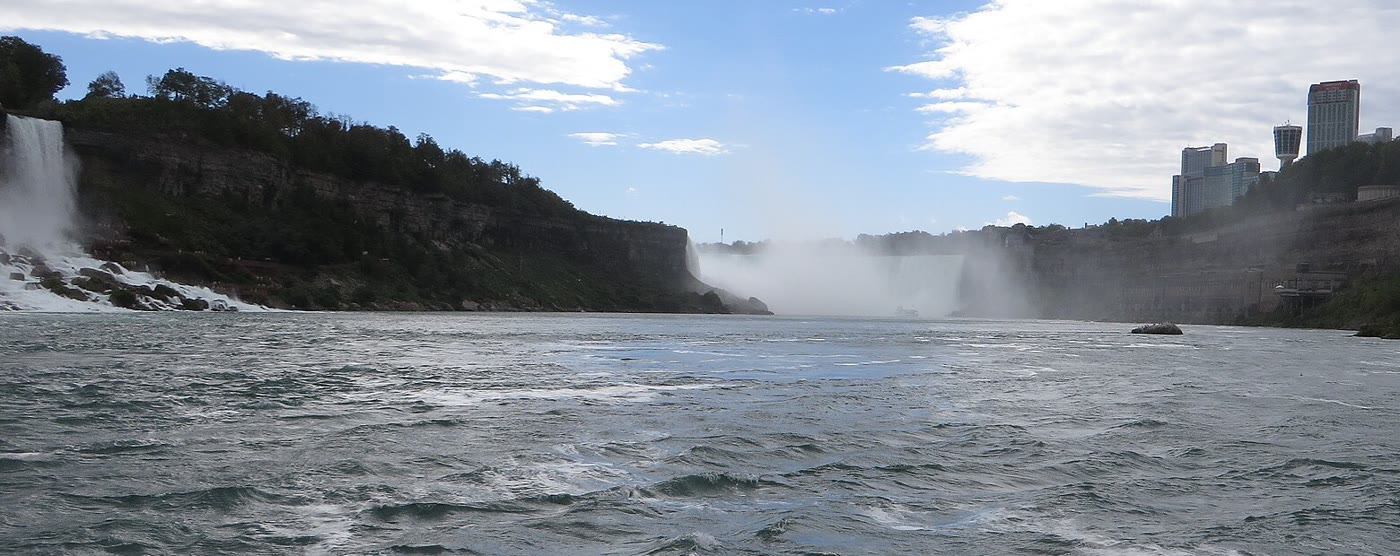
\includegraphics[width=\linewidth]{images/book5/b3-niagara-gorge.jpg}

{\scriptsize नायगारा गॉर्ज, ऊपर की ओर, धुंध में लिपटे घोड़े की नाल प्रपात की ओर देखता हुआ, उसकी
अमेरिकी प्रपात बाईं किनारी पर। फ़ोटो: केन लंड,
CC BY-SA 2.0 (काटा गया)।}
\end{minipage}
\end{inthefield}
% ledger: ijc18:niagara, photo:b3-niagara-gorge


\section{हिमनदीय अपरदन}\label{sec:b3:quantitative-geomorphology:glacial}

हिमनद अपने तल पर सरकते हुए (आधारी सर्पण,
अध्याय~\ref{ch:b3:glaciology}) में, वह उसे घर्षण द्वारा अपरदित करता है: बर्फ़ में फँसा मलबा
चट्टान को खुरचता है, और उखाड़ने द्वारा, जब वह दरारों से ढीले हुए खंडों को खींच लेता है।
दोनों सरकने की गति के अनुपात में बढ़ते हैं।

\begin{definition}[हिमनदीय अपरदन नियम]\label{def:b3:quantitative-geomorphology:glacial}
एक \emph{हिमनदीय अपरदन नियम}\index{हिमनदीय अपरदन नियम} वह संबंध है जो हिमनद के तल की
अपरदन दर को $E = K_G\,u_s^{\,l}$ द्वारा देता है, जहाँ $u_s$
सरकने की गति है, $K_G$ एक गुणांक और $l$ एक घातांक।
\end{definition}

भूदृश्य मॉडल प्रायः $l = 1$ लेते हैं, और उपयोग में 1 और 2 के बीच के मान भी आते हैं।
38 हिमनदों का एक संकलन, जिसकी अपरदन दरें पाँच कोटि के
परिमाण तक फैली हैं, यह पाता है कि अपरदन सरकने की गति से सहसंबद्ध है, जिसमें $l = 0.65$ और
$K_G = 10^{-4}$ है, जब $E$ मीटर प्रति वर्ष में हो: अपरदन सबसे तेज़ उन शीतोष्ण हिमनदों के नीचे होता है
जिन्हें प्रचुर हिमपात पोषित करता है और जो तेज़ी से सरकते हैं। चूँकि बर्फ़ घाटी की अक्ष के साथ सबसे मोटी
और सबसे तेज़ चलती है, इसलिए घाटी का तल किनारों की तुलना में अधिक
गहरा होता है, और घाटी अपना U आकार ग्रहण करती है।
% ledger: cook20:glacial

\begin{definition}[हिमनदीय आरी]\label{def:b3:quantitative-geomorphology:buzzsaw}
\emph{हिमनदीय आरी}\index{हिमनदीय आरी} हिमनदों द्वारा पर्वत-श्रेणी की ऊँचाई पर
लगाई गई सीमा है: जहाँ चट्टान उस ऊँचाई से ऊपर उठती है
जिस पर हिमनद बनते हैं, वे उसे उतनी ही तेज़ी से अपरदित करते हैं जितनी तेज़ी से वह उठती है, उत्थान दर चाहे
जो हो, ताकि शिखर और माध्य ऊँचाई उसी ऊँचाई के आसपास एकत्र हों।
\end{definition}

\section{विवर्तनिकी और अपरदन}\label{sec:b3:quantitative-geomorphology:tectonics}

\begin{definition}[स्थलाकृतिक स्थायी अवस्था]\label{def:b3:quantitative-geomorphology:steady-state}
कोई भूदृश्य \emph{स्थलाकृतिक स्थायी अवस्था}\index{स्थलाकृतिक स्थायी अवस्था} में होता है
जब हर जगह उसकी अपरदन दर चट्टान के उत्थान दर के बराबर हो, इसलिए
उसकी ऊँचाइयाँ नहीं बदलतीं, भले ही उसमें से चट्टान गुज़रती रहे।
\end{definition}

भिन्न-भिन्न समय-अवधियों पर मापी गई दरें इस अवस्था की जाँच करती हैं। \omterm{def:b3:advanced-geochronology:cosmogenic}{ब्रह्मांडजनित
नाभिक} नदी की रेत में जल-निकास द्रोणी की माध्य अपरदन दर देते हैं, उस समय पर
जिसमें उनके उत्पादन की क्षीणन लंबाई की कोटि की एक परत, लगभग
\qty{55}{cm} चट्टान, हटाई जा सके; \omterm{def:b3:orogenic-wedges:thermochronology}{ऊष्मकालमापी} और उनके \omterm{def:b3:orogenic-wedges:age-elevation}{आयु--ऊँचाई संबंध}
लाखों वर्षों पर उत्खनन-दर देते हैं। जहाँ ये दोनों एक-दूसरे से और उत्थान दर से मेल खाते हैं,
भूदृश्य संभवतः \omterm{def:b3:quantitative-geomorphology:steady-profile}{स्थायी अवस्था} में है; और जहाँ
अल्पकालिक दर निचले भाग में शीर्ष-धाराओं की तुलना में तेज़ हो,
वहाँ \omterm{def:b3:quantitative-geomorphology:knickpoint}{निकपॉइंट} गुज़र रहा है। चट्टान हटाने से स्थलमंडल का भार भी घटता है,
और वह उसके प्रत्युत्तर में ऊपर उठता है।
% ledger: zech04:exposure

\begin{definition}[अपरदनी समस्थितिक उत्क्षेप]\label{def:b3:quantitative-geomorphology:rebound}
\emph{अपरदनी समस्थितिक उत्क्षेप}\index{अपरदनी समस्थितिक उत्क्षेप} वह है
जिसमें समस्थितिक संतुलन में किसी क्षेत्र की चट्टान-सतह का उत्थान होता है
जो अपरदन द्वारा हटाए गए द्रव्यमान के प्रत्युत्तर में होता है।
\end{definition}

\begin{proposition}[घाटियों के गहरे होने पर शिखर उठते हैं]\label{prop:b3:quantitative-geomorphology:rebound}
एयरी समस्थिति में, घनत्व $\rho_c$ की भूपर्पटी घनत्व
$\rho_m$ के प्रावार के ऊपर हो, तो किसी क्षेत्र से भूपर्पटी की माध्य मोटाई $\bar e$ हटाने पर
पूरा क्षेत्र $(\rho_c/\rho_m)\,\bar e$ से ऊपर उठता है। यदि अपरदन केवल घाटियों तक सीमित हो,
तो बिना अपरदित शिखर उतना ही ऊपर उठते हैं, जबकि माध्य
सतह केवल $(1 - \rho_c/\rho_m)\,\bar e$ से नीचे गिरती है।
\end{proposition}

\begin{proof}
प्रतिपूर्ति के लिए आवश्यक है कि एक निश्चित गहराई के ऊपर हर स्तंभ का द्रव्यमान
वही रहे। भूपर्पटी की मोटाई $\bar e$ हटाना, क्षेत्र पर औसत लेकर,
प्रतिपूर्ति के क्षेत्र पर, प्रति एकक क्षेत्र द्रव्यमान को $\rho_c \bar e$ से घटाता है;
उसकी पूर्ति के लिए गहराई पर प्रावार का अंदर बहना आवश्यक है, जो स्तंभ का आधार
स्तंभ और उस पर की हर वस्तु को $\delta$ से ऊपर उठाता है, जहाँ $\rho_m \delta = \rho_c \bar
e$ है। बिना चट्टान खोए शिखर $\delta$ से ऊपर उठता है; माध्य सतह
$\bar e$ खोती है और $\delta$ प्राप्त करती है।
\end{proof}

संदर्भ पृथ्वी मॉडल की भूपर्पटी का मोटाई-भारित घनत्व
\qty{2.72}{g/cm^3} है, और उसके मोहो के नीचे प्रावार का \qty{3.38}{g/cm^3},
अनुपात 0.80 है: अपरदित हर सौ मीटर चट्टान में से माध्य सतह
केवल बीस खोती है। इसी प्रकार किसी पुराने पठार का गहरा अधःकर्तन उसके
शिखरों को ऊपर उठा सकता है, भले ही पठार घिसता जाए।
% ledger: prem:crust-mantle-ratio

\begin{omfigure}
\begin{tikzpicture}[x=0.6cm, y=0.6cm, font=\scriptsize]
\begin{scope}
\fill[omDef!12] (0,0) rectangle (8,4);
\draw[thick] (0,4) -- (8,4);
\draw[densely dashed] (0,0) -- (8,0);
\node[anchor=north] at (4,-0.1) {भूपर्पटी का आधार};
\node at (4,2) {भूपर्पटी $\rho_c$};
\node at (4,-1.2) {प्रावार $\rho_m$};
\node[anchor=south] at (4,4.1) {पहले};
\end{scope}
\begin{scope}[xshift=6.2cm]
\fill[omDef!12] (0,0.8) -- (0,4.8) -- (1.4,4.8) -- (2.0,2.4) -- (2.6,4.8) -- (5.4,4.8) -- (6.0,2.4) -- (6.6,4.8) -- (8,4.8) -- (8,0.8) -- cycle;
\draw[thick] (0,4.8) -- (1.4,4.8) -- (2.0,2.4) -- (2.6,4.8) -- (5.4,4.8) -- (6.0,2.4) -- (6.6,4.8) -- (8,4.8);
\draw[black!50, densely dashed] (0,4) -- (8,4);
\draw[densely dashed] (0,0.8) -- (8,0.8);
\draw[densely dashed, black!40] (0,0) -- (8,0);
\draw[<->, omThm] (8.3,4.05) -- (8.3,4.75) node[midway, right] {$\delta$};
\draw[<->, omThm] (8.3,0.05) -- (8.3,0.75) node[midway, right] {$\delta$};
\node[anchor=west, font=\scriptsize] at (8.1,2.4) {$\delta = (\rho_c/\rho_m)\,\bar e$};
\node[anchor=south] at (4,5.0) {अधःकर्तन के बाद};
\node[anchor=north] at (2.0,2.3) {घाटी};
\end{scope}
\end{tikzpicture}

\par\smallskip{\small \omterm{def:b3:quantitative-geomorphology:rebound}{अपरदनी समस्थितिक उत्क्षेप}, योजनाबद्ध चित्र। घाटियाँ
काटने से औसत मोटाई $\bar e$ की भूपर्पटी हट जाती है; स्तंभ
अपने आधार पर और अपने अछूते शिखरों पर $\delta = (\rho_c/\rho_m)\bar e$ जितना उठ जाता है
(धूसर बिंदीदार रेखा पुरानी सतह है)।}\label{fig:b3:quantitative-geomorphology:rebound}
\end{omfigure}

\section{अभ्यास}

\begin{exercise}[$\star$]\label{exo:b3:quantitative-geomorphology:1}
विस्थापन \qty{4}{m} ($a = \qty{2}{m}$) वाला एक तटरेखा कगार दूर-क्षेत्र की
0.04 ढाल पर खड़ा है, और इसकी सबसे तीखी प्रवणता अब 0.30 है।
पहले $\kappa t$ परिकलित कीजिए, फिर $\kappa = \qty{5e-3}{m^2/yr}$ लेकर कगार की आयु ज्ञात कीजिए।
\end{exercise}
% ledger: whipple04:scarp-erf, whipple04:scarp-kappa

\begin{exercise}[$\star$]\label{exo:b3:quantitative-geomorphology:2}
एक लिडार सर्वेक्षण से एक कटक के शिखर पर वक्रता \qty{-0.012}{m^{-1}} मिलती है,
जिसकी विसरणशीलता \qty{4e-3}{m^2/yr} है। इसकी अपरदन दर
\unit{mm/yr} में परिकलित कीजिए, और इसके शिखर तथा
\qty{80}{m} दूर की वाहिकाओं के बीच का उच्चावच ज्ञात कीजिए, \omterm{def:b3:quantitative-geomorphology:steady-profile}{स्थायी अवस्था} मानकर।
\end{exercise}

\begin{exercise}[$\star$]\label{exo:b3:quantitative-geomorphology:3}
$m = 0.5$, $n = 1$ और $K = \qty{2e-6}{yr^{-1}}$ लेकर
\qty{25}{km^2} क्षेत्रफल का जल-निकास करने वाली, 0.01 प्रवणता वाली नदी की अधःकर्तन दर परिकलित कीजिए,
और $K$ की इकाइयाँ सामान्य $m$ और $n$ के लिए क्या हैं?
\end{exercise}

\begin{exercise}[$\star$]\label{exo:b3:quantitative-geomorphology:4}
तीन नदियों में \omterm{def:b3:quantitative-geomorphology:knickpoint}{निकपॉइंट} दिखाई देते हैं: (क) जहाँ बलुआ पत्थर का संस्तर शेल में कटी
घाटी को पार करता है; (ख) जहाँ नदी एक सक्रिय सामान्य भ्रंश को निचली भित्ति से
ऊपरी भित्ति की ओर पार करती है; (ग) किसी द्रोणी की हर नदी में, लगभग एक ही ऊँचाई पर,
एक भूकंप में ऊपर उठे तट से कुछ किलोमीटर ऊपर।
कौन-से स्थिर हैं और कौन-से स्थानांतरित होंगे?
\end{exercise}

\begin{exercise}[$\star\star$]\label{exo:b3:quantitative-geomorphology:5}
$m = 1$ और $n = 2$ के लिए $\theta$ और वह स्थायी प्रवणता परिकलित कीजिए जहाँ $A =
\qty{10}{km^2}$, $U = \qty{0.1}{mm/yr}$ और $K = 10^{-9}$ लेकर, जहाँ मीटर और
वर्ष इकाइयाँ हैं।
यदि $U$ दोगुना हो तो तीव्रता किस गुणक से बदलती है? $n =
1$ की स्थिति से तुलना कीजिए।
\end{exercise}

\begin{exercise}[$\star\star$]\label{exo:b3:quantitative-geomorphology:6}
नदी का जल-निकास क्षेत्र, विभाजक से दूरी $d$ के साथ $A =
c\,d^{h}$ के रूप में बढ़ता है। दिखाइए कि निर्गम से, जो $d = L$ पर है, ऊपर की ओर मापने पर
\[
\chi(d) = \frac{A_0^{\theta}}{c^{\theta}}\,\frac{L^{p} - d^{p}}{p},
\qquad p = 1 - h\theta ,
\]
$c = 2$ (SI), $h = 1.8$, $\theta = 0.45$ और $A_0 =
\qty{1}{km^2}$, $L = \qty{20}{km}$ और $d = \qty{5}{km}$ के लिए इसका मान परिकलित कीजिए।
\end{exercise}

\begin{exercise}[$\star\star$]\label{exo:b3:quantitative-geomorphology:7}
$n = 1$, $m = 0.5$ और $K = \qty{2e-6}{yr^{-1}}$ लेकर, एक \omterm{def:b3:quantitative-geomorphology:knickpoint}{निकपॉइंट} की चाल,
जहाँ $A = \qty{100}{km^2}$ है, m/kyr में, और
उस चाल से \qty{5}{km} दूरी तय करने में लगने वाला समय भी परिकलित कीजिए। वास्तव में यह
अधिक समय क्यों लेता है?
\end{exercise}

\begin{exercise}[$\star\star$]\label{exo:b3:quantitative-geomorphology:8}
\qty{600}{m} गहरी घाटियाँ, जो औसतन \qty{40}{\percent} क्षेत्रफल घेरती हैं,
एक पठार के क्षेत्रफल का, उसमें काटी गई हैं। $\rho_c/\rho_m = 0.80$ लेकर
अपरदित औसत मोटाई, शिखरों का उत्थान और
औसत ऊँचाई का परिवर्तन परिकलित कीजिए।
\end{exercise}
% ledger: prem:crust-mantle-ratio

\begin{exercise}[$\star\star$]\label{exo:b3:quantitative-geomorphology:9}
एक \omterm{def:b3:quantitative-geomorphology:soil-production}{मृदा उत्पादन फलन} के लिए $P_0 = \qty{0.3}{mm/yr}$ और $h_0 =
\qty{0.5}{m}$ है। अपरदन दर
\qty{0.05}{mm/yr} और \qty{0.2}{mm/yr} पर स्थायी मृदा मोटाई परिकलित कीजिए। \qty{0.4}{mm/yr} पर
क्या होता है?
\end{exercise}

\begin{exercise}[$\star\star\star$]\label{exo:b3:quantitative-geomorphology:10}
\omterm{def:b3:quantitative-geomorphology:steady-profile}{स्थायी अवस्था} में एक पहाड़ी $E = \qty{0.1}{mm/yr}$ दर से अपरदित होती है, $\kappa =
\qty{5e-3}{m^2/yr}$ है, और क्रांतिक प्रवणता का अरैखिक नियम है,
जिसमें अभ्यास के लिए $S_c = 1.2$ लीजिए। दिखाइए कि विभाजक से $x$ दूरी पर फ़्लक्स
$E x$ है, प्रवणता के लिए हल कीजिए और इसे 20, 50, 100 और
\qty{200}{m} पर परिकलित कीजिए। रैखिक विसरण से तुलना कीजिए और पहाड़ी
के आकार का वर्णन कीजिए।
\end{exercise}

\begin{exercise}[$\star\star\star$]\label{exo:b3:quantitative-geomorphology:11}
दिखाइए कि नदी-जाल का, उसके निर्गम पर हुए परिवर्तन के प्रति अनुक्रिया-काल,
$n = 1$ के लिए, $\chi_h/(K A_0^m)$ है, जहाँ $\chi_h$ वाहिका-शीर्ष पर $\chi$ का
सबसे बड़ा मान है। चित्रों की पर्वतीय नदी के लिए इसे परिकलित कीजिए
($A_0 = \qty{1}{km^2}$, $m = 0.5$, $K = \qty{e-6}{yr^{-1}}$), पहले केवल
इसकी मुख्य धारा के लिए, जिसका शीर्ष $\chi = \qty{5464}{m}$ पर है, फिर पूरे जाल के लिए,
जिसका सबसे ऊँचा शीर्ष, सहायक नदी 1 पर, $\chi = \qty{7237}{m}$ पर है।
\end{exercise}

\begin{exercise}[$\star\star\star$]\label{exo:b3:quantitative-geomorphology:12}
$n = 1$ और एकसमान $U$ वाले जाल में, एक सहायक नदी चट्टान पर बहती है जो
शेष से दोगुनी अपरदनशील है ($2K$), अपने संगम से ऊपर, $\chi_j$ पर। दिखाइए कि
$(\chi, z)$ तल में इसकी स्थायी-अवस्था रेखा की प्रवणता, $\chi_j$ से ऊपर
मुख्य धारा की प्रवणता की आधी है, और निर्गम पर जन्मा एक \omterm{def:b3:quantitative-geomorphology:knickpoint}{निकपॉइंट}
जब मुख्य धारा का \omterm{def:b3:quantitative-geomorphology:knickpoint}{निकपॉइंट} $\chi_k > \chi_j$ पर होता है, तब उस सहायक नदी पर
$\chi = \chi_j + 2(\chi_k - \chi_j)$ वाले बिंदु तक पहुँच चुका होता है।
\end{exercise}

\section{समस्या: वार्डन नदी का जलप्रपात}

\begin{problem}[{सप्ताहांत समस्या --- एक काल्पनिक पर्वतीय नदी की रूपरेखा, तीव्रता और अपरदनशीलता,
और उसके जलप्रपात की आयु}]
\label{pb:b3:quantitative-geomorphology:1}
वार्डन पहाड़ियों के पश्चिम में, नदी शिस्ट की एक पर्वतीय भूमि का जल-निकास करती है, इससे पहले कि वह
मानचित्र में अपने पश्चिमी किनारे से, \qty{170}{m} की ऊँचाई पर प्रवेश करती है। उस बिंदु के, जो इसका निर्गम है, ऊपर
की ओर मुख्य धारा विभाजक से \qty{12}{km} लंबी है,
जल-निकास क्षेत्र $A = 4.5\,d^{1.7}$ (\unit{m^2}, $d$ विभाजक से मीटर में) के साथ,
और वाहिका-शीर्ष $d = \qty{300}{m}$ पर है। चट्टान-उत्थान की दर के रूप में
वार्डन नदी द्रोणी की, पुस्तक 3 (स्नातक वर्ष 1) में उसके भार से ज्ञात अनाच्छादन दर लीजिए,
जो \qty{43}{m/Myr} है। $n = 1$ और संदर्भ क्षेत्रफल $A_0 = \qty{1}{km^2}$ मान लीजिए।
मुख्य धारा पर, निर्गम के \qty{4.60}{km} ऊपर, \qty{25}{m} ऊँचा एक जलप्रपात
स्थित है। सभी मान काल्पनिक हैं।

\medskip\noindent\textbf{भाग I --- प्रोफ़ाइल।}
\begin{enumerate}
\item निर्गम पर और वाहिका-शीर्ष पर जल-निकास क्षेत्र परिकलित कीजिए।
\item जलप्रपात से दूर, \qty{200}{m} लंबे खंडों पर मापी गई प्रवणताएँ
  इस प्रकार हैं:

  \smallskip
  {\small\begin{tabular}{l*{6}{c}}
  $A$ (\unit{km^2}) & 0.388 & 0.587 & 0.888 & 1.345 & 2.036 & 3.082 \\
  $S$ & 0.06641 & 0.05026 & 0.04888 & 0.03322 & 0.03688 & 0.02688 \\[2pt]
  $A$ (\unit{km^2}) & 4.665 & 7.061 & 10.69 & 16.18 & 24.49 & 37.08 \\
  $S$ & 0.01921 & 0.01713 & 0.01545 & 0.01419 & 0.007922 & 0.007855
  \end{tabular}}

  \smallskip
  पहले और अंतिम बिंदुओं से \omterm{def:b3:quantitative-geomorphology:indices}{अवतलता सूचकांक} का अनुमान लगाइए।
\item $\log S$ बनाम $\log A$ की न्यूनतम वर्ग प्रवणता $-0.466$ है।
  क्या यह $\theta = 0.5$ के अनुरूप है?
\item $\theta_{\mathrm{ref}} = 0.5$ लेकर, पहले और अंतिम बिंदु के लिए $k_{sn} = S A^{0.5}$ ($A$
  \unit{m^2} में) परिकलित कीजिए, और बताइए कि बारह मानों का ज्यामितीय
  माध्य, \qty{45.1}{m}, क्या निरूपित करता है।
\item प्रवणताएँ उन्नयनों की तुलना में इतनी अधिक क्यों बिखरती हैं?
\item काई अभ्यास के सूत्र का उपयोग करके $\chi$ परिकलित कीजिए, $d =
  \qty{9.00}{km}$ पर, जो जलप्रपात के नीचे का एक बिंदु है।
\end{enumerate}

\medskip\noindent\textbf{भाग II --- प्रवणता और अपरदनशीलता।}
\begin{enumerate}[resume]
\item $d = \qty{9.00}{km}$ पर नदी \qty{193.4}{m} पर है। जलप्रपात के नीचे के
  काई आलेख की प्रवणता और \omterm{def:b3:quantitative-geomorphology:indices}{वाहिका ढाल-सूचकांक} $k_{sn}$ परिकलित कीजिए।
\item $k_{sn}$ का कौन-सा अनुमान, यह वाला या क्षेत्र-प्रवणता वाला, आप अधिक भरोसेमंद मानेंगे,
  और क्यों?
\item जलप्रपात के नीचे \omterm{def:b3:quantitative-geomorphology:steady-profile}{स्थायी अवस्था} मानकर, उत्थान दर से $K$
  परिकलित कीजिए।
\item जाँच कीजिए कि निर्गम पर अधःकर्तन दर, जिसकी प्रवणता
  0.00691 है, उत्थान दर के बराबर है।
\item निर्गम पर और जलप्रपात पर \omterm{def:b3:quantitative-geomorphology:knickpoint}{निकपॉइंट} का वेग
  m/kyr में परिकलित कीजिए।
\item स्थायी प्रोफ़ाइल पर वाहिका-शीर्ष की ऊँचाई
  और मुख्य धारा का उच्चावच परिकलित कीजिए।
\end{enumerate}

\medskip\noindent\textbf{भाग III --- जलप्रपात।}
\begin{enumerate}[resume]
\item $n = 1$ होने पर भी जलप्रपात ने \omterm{def:b3:quantitative-geomorphology:knickpoint}{आधार-तल} के गिरने की ऊँचाई
  क्यों बनाए रखी है?
\item जलप्रपात पर $\chi$ परिकलित कीजिए।
\item निर्गम से \omterm{def:b3:quantitative-geomorphology:knickpoint}{निकपॉइंट} की अपनी वर्तमान जगह तक पहुँचने में लगा समय
  परिकलित कीजिए।
\item अब से \qty{300}{kyr} बाद वह कहाँ होगा?
\item सहायक नदी 3 निर्गम के \qty{2.5}{km} ऊपर मुख्य धारा से मिलती है; इसकी
  लंबाई \qty{5}{km} है, और $A = 1.5\,s^{1.7}$ ($s$ उसके अपने विभाजक से) है।
  उसका जलप्रपात कहाँ होना चाहिए?
\item सहायक नदियाँ 1 और 2 मुख्य धारा से निर्गम के 8 और \qty{5}{km} ऊपर मिलती हैं
  समझाइए कि उनमें जलप्रपात क्यों नहीं है।
\end{enumerate}

\medskip\noindent\textbf{भाग IV --- ढाल और आयु।}
\begin{enumerate}[resume]
\item जलप्रपात के ऊपर एक लिडार सर्वेक्षण से शिखर-वक्रता
  \qty{-0.0086}{m^{-1}} मिलती है। $\kappa = \qty{5e-3}{m^2/yr}$ लेकर
  अपक्षरण दर परिकलित कीजिए और उसकी तुलना उत्थान दर से कीजिए।
\item ढाल लगभग \qty{150}{m} लंबे हैं। भाग III में मिली आयु की
  तुलना उनके प्रतिक्रिया-काल $L^2/\kappa$ से कीजिए।
\item आज जलप्रपात के नीचे के ढालों का वर्णन कीजिए,
  और वे कैसे बदलेंगे।
\item उत्थान दर \qty{20}{\percent} तक ज्ञात है।
  आयु का परास दीजिए।
\item यदि $n$ 2 होता, तो जलप्रपात कैसे विकसित हुआ होता?
\item \omterm{def:b3:quantitative-geomorphology:knickpoint}{आधार-तल} के गिरने की आयु दीजिए।
\end{enumerate}
\end{problem}
% ledger: whipple04:steepness, whipple04:scarp-kappa
